% StateForge —— NDSS 论文初稿 (2026-09-19)
% 格式:NDSS(15 页正文 + 参考);需要 ndss.sty(NDSS 官方模板)放入本目录
% 编译:pdflatex main && pdflatex main
% 所有 \planned{} 为待实验数据填充位,填充前不得删除标记
\documentclass[letterpaper,twocolumn,10pt]{article}
\usepackage{ndss}  % NDSS 官方模板样式;获取:NDSS 作者工具包(需放入本目录)
\usepackage{amsmath,amssymb,graphicx}
\usepackage{tikz}
\usetikzlibrary{arrows.meta,positioning,fit,backgrounds,calc}
\usepackage{xcolor}
\usepackage[colorlinks=true,linkcolor=blue,citecolor=blue]{hyperref}

\newcommand{\planned}[1]{\textcolor{red}{[PLANNED: #1]}}
\newcommand{\sys}{\textsc{StateForge}}

\begin{document}

\date{}
\title{\Large \bf StateForge: Recovering and Navigating Application State Spaces\\ for Deep Web Vulnerability Discovery}
\author{{\normalsize Anonymous submission}\\[-2mm]
{\normalsize NDSS review draft, compiled \today}}
\maketitle

\begin{abstract}
Many severe web application vulnerabilities---post-authentication remote code execution, stored (second-order) injection, privilege-escalation and workflow-bypass chains---are gated not by code reachability but by \emph{application state}: they trigger only after authentication is established, a payload has been persisted, or a one-shot flag has flipped. Directed fuzzers steer by code-space distance and must pre-provision state by hand; snapshot fuzzers restore state cheaply but neither model nor direct it. We argue that the relevant search space for these \emph{deep} vulnerabilities is the state space, and we present \sys{}, a system that operates in it end to end. \sys{} (i)~recovers a security-relevant state space from source code by combining static candidate mining with candidate-anchored LLM semantic lifting---the LLM interprets statically enumerated candidates but cannot invent states or transitions; (ii)~directs exploration toward \emph{new states}---the unvisited frontier of the recovered space---with deterministic planning constructing the gate-opening chains and mutation exploring beyond the model, so that each state gate crossed unlocks the deeper code regions behind it and classical code coverage, our reported objective, improves as a consequence; and (iii)~makes state construction cheap and repeatable through fork-based copy-on-write epochs with bit-exact file-database templates, with checkpoint placement itself scheduled by state properties. Runtime annotations in an instrumented interpreter serve as passing oracles---never as the steering signal---so no vulnerability report is required a priori. Preliminary results: all five state-gated vulnerability classes are reached by planned chains on a controlled target (10/10 goal$\times$variant matrix, including a payment bypass that skips payment entirely); identical verdicts hold through both persistent and snapshot executors; restore costs ${\sim}0.7$\,ms independent of chain depth; LLM labels agree with hand-written ground truth on 6/6 state variables and drafted annotations match hand-written policies at 1.0 recall. The full three-baseline campaign is \planned{underway}.
\end{abstract}

\section{Introduction}
\label{sec:intro}

Web applications are stateful machines. A request does not merely invoke code---it \emph{transitions} application state: rows are created, session identities are established, one-shot flags flip, workflow enums advance, and payloads are persisted for later consumption. A large and severe class of vulnerabilities is gated behind such transitions:

\begin{itemize}
\item \textbf{Post-authentication RCE.} A command-execution or file-handling sink fires only for authenticated principals; the pre-auth attack surface sanitizes it away.
\item \textbf{Second-order (stored) injection.} A payload stored by one request (a comment, a profile field) becomes an input consumed by a later request at a dangerous use point; no single request is malicious on its own.
\item \textbf{State-machine and one-shot violations.} Orders ship without payment; coupons redeem twice; privileges escalate through a role field that anyone may write.
\end{itemize}

These vulnerabilities defeat both families of state-of-the-art web fuzzers for a structural reason we summarize as: \emph{code distance is not state distance}. The difficulty is empirical, not rhetorical: recent measurement reports that state-of-the-art baselines fail on all attacks requiring more than two state-setting requests, even when equipped with the necessary payloads~\cite{ariadne}.

\textbf{Directed fuzzers fail on the far side of the state gate.} Tools in the AFLGo~\cite{aflgo}--Predator~\cite{predator} lineage prioritize inputs by code-space proximity to a target location. For a second-order flaw, the use point executes on \emph{every} request---its control-flow distance is essentially zero---while its distance in state space (payload stored, session valid) is several transitions away. Code-directed energy is spent on inputs that approach the sink yet never enter the required state. The state itself is provisioned by hand: Predator's evaluation provides the crawler with valid credentials~\cite{predator}, and its authors note that errors manifesting only under specific states may remain undetected.

\textbf{Snapshot fuzzers restore state but cannot navigate it.} Atropos~\cite{atropos} restores full-system snapshots so that state accumulates across inputs within an epoch, and we have independently verified its central claim: second-order detection requires \emph{both} a use-point oracle \emph{and} a state chain. But without a model of the state space there is no direction signal: state accumulates blindly, checkpoints are placed by heuristic (e.g., after login), and whether a target state is reachable---or \emph{why} it is not---is invisible.

\textbf{This paper.} We present \sys{}, which closes the loop between modeling, direction, and reset (Figure~\ref{fig:overview}):

\begin{enumerate}
\item \textbf{Semantic state recovery (\S\ref{sec:recovery}).} Static pattern mining produces \emph{state candidates}---unjudged facts with code anchors. An LLM performs \emph{candidate-anchored semantic lifting}: each candidate is classified into one of six security semantics (\texttt{authn}, \texttt{authz}, \texttt{ownership}, \texttt{money}, \texttt{workflow}, \texttt{single-use}) with an auditable rationale, under enum-constrained, schema-validated output. A published deterministic selector admits labeled candidates into a \emph{Security State Transition Graph} (SSTG) whose legal transitions derive from guard--effect pairing in code. The model has a lifecycle: runtime calibration, and LLM-assisted repair---as execution-adjudicated hypotheses---when targets remain unreachable.
\item \textbf{New-state-directed exploration (\S\ref{sec:navigate}).} The navigation target is the \emph{unvisited state frontier}, not a code location---and thus no vulnerability report is required a priori. A backward planner constructs gate-opening chains toward frontier states (dropping preconditions that static analysis observes to be flag-conditional---the attack-hypothesis generator); a fuzzer explores beyond the model with \emph{state novelty} as its direction signal: at epoch end, read-back observations are diffed against known state atoms; new atoms advance the frontier, reward seeds, repair the graph, and nominate checkpoints. Code coverage---the classical objective---improves as gates unlock the regions behind them; annotations judge violations encountered along the way and never steer.
\item \textbf{State-aware snapshot execution (\S\ref{sec:snapshot}).} One chain equals one epoch equals one forked copy-on-write leaf; a bit-exact file-database template restores disk to the checkpoint's page cache exactly. Nested checkpoints let goal families fork from depth $k$ rather than replay prefixes; placement is scheduled by a state score (security relevance, prefix reuse, rebuild cost, novelty).
\item \textbf{Annotations as targets and oracles (\S\ref{sec:annotations}).} Each annotated guard site in the instrumented interpreter is simultaneously a violation oracle and a \emph{target specification}---a (state gate $\times$ sink) pair. The same annotations drive our B1 baseline (oracle only) and \sys{} (oracle plus target-driven construction), isolating the state layer's contribution; because annotations are machine-draftable from the recovered state machine (1.0 recall against hand-written policies), so is the target set.
\end{enumerate}

\textbf{Contributions.}
\begin{itemize}
\item A formulation of deep web vulnerability discovery as reachability in a recovered application state space, with a five-dimension state-space definition organized by storage location (\S\ref{sec:formulation}).
\item A candidate-anchored semantic lifting protocol that confines the LLM to interpreting statically enumerated facts---preserving interpretability and reproducibility---within a model lifecycle of recovery, calibration, and repair (\S\ref{sec:recovery}).
\item The unification of deterministic planning (exploitation, state-distance directed) and fuzzing (exploration, state-novelty feedback) on one graph, replacing code distance as the direction signal (\S\ref{sec:navigate}).
\item Snapshot scheduling by state properties atop fork COW and bit-exact database templates (\S\ref{sec:snapshot}).
\item A working implementation and preliminary evidence: 10/10 goal$\times$variant reachability with identical verdicts under two executors, sub-millisecond depth-independent restore, exact epoch isolation, and labeling/annotation quality matching ground truth (\S\ref{sec:eval}); the full three-baseline campaign is \planned{underway}.
\end{itemize}

\section{Background and Motivation}
\label{sec:motivation}

\subsection{State-gated vulnerabilities}
We use \emph{state-gated} for vulnerabilities whose triggering condition is a predicate over application state rather than (only) the content of a single request. Three families anchor our study. Post-authentication RCE and injection: the sink is reachable in code for all callers, but sanitization or dispatch routes only authenticated principals into it. Second-order injection: the payload crosses a persistence boundary between requests; the attacker's request is innocuous at storage time and the consuming request is innocuous without the stored value. Workflow and one-shot violations: business-logic preconditions (payment before shipping; single redemption) are enforced by state checks that a missing check silently disables.

\subsection{What each family of tools is missing}
\textbf{Coverage-guided and code-directed fuzzing.} Witcher~\cite{witcher} pairs coverage feedback with annotation-style checks; Predator~\cite{predator} validates static reports with block-distance direction, entry-URL backward analysis, branch-derived parameter corpora, and runtime edge supplementation through selective PHP-opcode instrumentation. Both operate in code space. Predator's instrumentation of an \emph{augmented interpreter} for feedback is instructive---our runtime substrate is likewise an augmented interpreter (ANOTA's instrumented CPython~\cite{anota}), but it yields \emph{semantic} observations (annotation events, state read-backs) rather than block distances, and our direction signal lives in the state graph. Crucially, Predator's sessions are pre-provisioned with valid credentials~\cite{predator}; authentication is not something its fuzzer \emph{constructs}. SDFuzz~\cite{sdfuzz} drives by target \emph{states} in kernels---the closest conceptual relative---but its states are manually specified, whereas we recover application-semantic states from source. ChatAFL~\cite{chatafl} learns protocol state machines with LLM assistance and generates seeds; our states are application-semantic (database, workflow, session) and our LLM repairs the graph rather than synthesizing inputs.

\textbf{Snapshot fuzzing.} Atropos~\cite{atropos} restores snapshots between epochs and shows---and our independent port to process-level snapshots confirms---that second-order detection equals the product of a use-point oracle and a state chain: with the oracle fixed, per-input restoration yields no detection while epoch-level chaining detects. But Atropos accumulates state blindly: no model of what states exist, no distance signal toward targets, no explanation of unreachability, and heuristic checkpoint placement. \sys{} supplies exactly these: the SSTG provides the map, the planner the route, the novelty feedback the frontier, and the state score the checkpoint policy. Orthogonally, Ariadne~\cite{ariadne} performs \emph{forensic} reconstruction: given a detected terminal attack request, it recovers the prerequisite state-setting sequence via goal-oriented search with a state-distance metric derived from traffic data. Our work is complementary---we discover attacks before they occur, assume no attack or report as input, and recover the state model from source code rather than runtime logs.

\subsection{A motivating walkthrough}
Consider our controlled application's payment-bypass flaw. The ship endpoint contains a check \texttt{if order["status"] != "PAID": reject}, wrapped in a runtime feature flag (single source, guarded/unguarded variants). A code-directed fuzzer sees the ship handler at near-zero distance and fires unauthenticated requests at it---all rejected with 401/409. Reaching the flaw requires a four-deep state chain: \texttt{register} (produces a user), \texttt{login} (produces a session), \texttt{create} (produces \texttt{Order.status=CREATED} bound to object id $\theta$), then \texttt{ship} under the attack hypothesis that the flag-conditional precondition is absent. Our planner emits exactly this chain---notably \emph{without} the payment step---from the recovered SSTG, and execution adjudicates: the unguarded variant reaches \texttt{SHIPPED} with \texttt{paid\_amount=0} (hit), the guarded variant blocks at ship (409). The hypothesis itself is machine-generable: static analysis observes the precondition's flag-conditionality. The question is not whether such chains exist---it is who can find them, and at what cost.

\section{Overview and Problem Formulation}
\label{sec:formulation}

\textbf{State space.} Let $V$ be the security-relevant projection of application state variables. We organize $V$ by \emph{storage location}, because storage determines both observability and controllability:

\begin{itemize}
\item[(i)] \emph{Session/token state}: authenticated identity, role claims, CSRF nonces. Observed via identity endpoints; controlled by client-held credentials (the binding $\theta$ from symbolic to runtime objects).
\item[(ii)] \emph{Persistent data state}: row existence, enum fields, one-shot flags, \emph{stored payloads}, ownership bindings. Observed via read-back endpoints; written by actions and reset by database templates.
\item[(iii)] \emph{Configuration state}: feature flags selecting attack-surface quadrants. Statically visible; selected by variant.
\item[(iv)] \emph{Process memory state}: globals, caches, pools. Not statically observable; reset wholesale by fork COW.
\item[(v)] \emph{File state}: application-written files. Reset by template extension (future work).
\end{itemize}

We model (i)--(iii)---the statically recoverable dimensions, including tainted-value variables whose domains are payload spaces---and reset (iv)--(v) wholesale: \emph{we model everything statically recoverable and reset the rest.}

\textbf{Actions, regions, depth.} An HTTP request is a partial transition $a: S \rightharpoonup S$. A vulnerability region $B \subseteq S$ is a state gate crossed with a sink (e.g., $\{\texttt{authed}\}\times\texttt{rce\_sink}$; $\{\texttt{payload\_stored}\}\times\texttt{use\_point}$), or an illegal transition. The \emph{depth} $d(B)$ is the minimum number of state-transitioning actions from the initial state $S_0$ to $B$. The SSTG is the AND/OR navigation projection of $S$ over security-relevant atoms; planning is route search; epochs are state rollback.

\textbf{Detection.} A finding requires
\begin{equation}
\mathrm{Reach}(B) \wedge \mathrm{Violation}(\Phi),
\end{equation}
some execution reaching $B$ and the oracle $\Phi$ firing at the sink---the conjunction our second-order measurement instantiates.

\textbf{Threat model.} We analyze server source available to the defender (white-box), target developer-introduced logic flaws in the application under its real stack, and treat the annotated oracle as trusted. Finding confirmations require reproducible chains; we do not claim zero-day collection at scale in this draft.

\section{Design}
\label{sec:design}

Figure~\ref{fig:overview} presents the architecture; \S\ref{sec:recovery}--\ref{sec:annotations} detail each stage and its rationale.

\begin{figure*}[t]
\centering
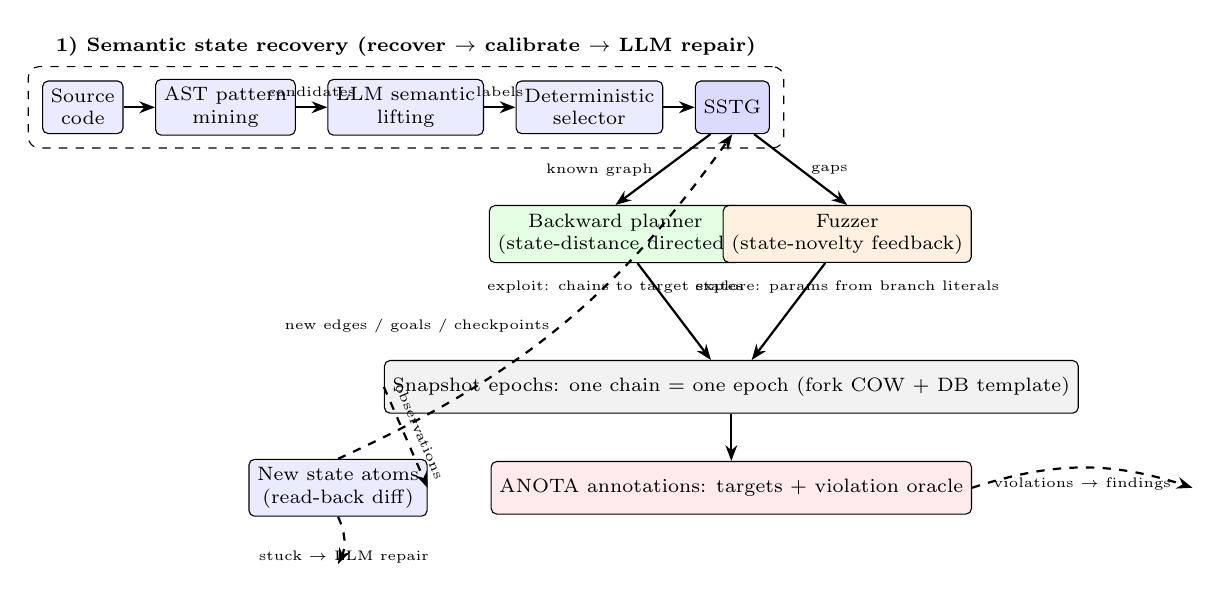
\begin{tikzpicture}[
  font=\scriptsize,
  box/.style={draw, rounded corners=2pt, align=center, inner sep=3pt, minimum height=1.9em},
  phase/.style={draw, dashed, rounded corners=4pt, inner sep=5pt},
  arr/.style={-{Stealth[length=2mm]}, thick},
  fbk/.style={-{Stealth[length=2mm]}, thick, dashed}
]
% Phase 1: recovery
\node[box, fill=blue!8] (ast) {Source\\code};
\node[box, fill=blue!8, right=4mm of ast] (cand) {AST pattern\\mining};
\node[box, fill=blue!8, right=4mm of cand] (llm) {LLM semantic\\lifting};
\node[box, fill=blue!8, right=4mm of llm] (sel) {Deterministic\\selector};
\node[box, fill=blue!14, right=4mm of sel] (sstg) {SSTG};
\draw[arr] (ast) -- (cand);
\draw[arr] (cand) -- node[above, font=\tiny]{candidates} (llm);
\draw[arr] (llm) -- node[above, font=\tiny]{labels} (sel);
\draw[arr] (sel) -- (sstg);
\begin{pgfonlayer}{background}
\node[phase, fit=(ast)(sstg), label={[font=\scriptsize\bfseries]above:1) Semantic state recovery (recover $\rightarrow$ calibrate $\rightarrow$ LLM repair)}] {};
\end{pgfonlayer}

% Phase 2: exploit / explore
\node[box, fill=green!10, below left=9mm and -6mm of sstg] (planner) {Backward planner\\(state-distance directed)};
\node[box, fill=orange!12, below right=9mm and -6mm of sstg] (fuzzer) {Fuzzer\\(state-novelty feedback)};
\draw[arr] (sstg.south west) ++(2mm,0) -- (planner.north) node[midway, left, font=\tiny]{known graph};
\draw[arr] (sstg.south east) ++(-2mm,0) -- (fuzzer.north) node[midway, right, font=\tiny]{gaps};
\node[font=\tiny, below=1mm of planner] {exploit: chains to target states};
\node[font=\tiny, below=1mm of fuzzer] {explore: params from branch literals};

% Phase 3: execution
\node[box, fill=gray!10, below=16mm of $(planner)!0.5!(fuzzer)$] (epoch) {Snapshot epochs: one chain = one epoch (fork COW + DB template)};
\draw[arr] (planner) -- (epoch);
\draw[arr] (fuzzer) -- (epoch);

% Phase 4: oracle
\node[box, fill=red!8, below=6mm of epoch] (anota) {ANOTA annotations: targets $+$ violation oracle};
\draw[arr] (epoch) -- (anota);

% Feedback
\node[box, fill=blue!8, left=8mm of anota] (newst) {New state atoms\\(read-back diff)};
\draw[fbk] (anota.east) to[bend left=18] node[below, font=\tiny]{violations $\rightarrow$ findings} ++(28mm,0);
\draw[fbk] (epoch.west) -- node[above, font=\tiny, sloped]{observations} (newst.east);
\draw[fbk] (newst.north) to[bend right=15] node[left, font=\tiny]{new edges / goals / checkpoints} (sstg.south);
\draw[fbk] (newst.south) to[bend left=25] node[below, font=\tiny]{stuck $\rightarrow$ LLM repair} ++(0,-6mm);
\end{tikzpicture}
\caption{\sys{} overview. Static analysis mines unjudged candidate facts; the LLM lifts them into security semantics; a deterministic selector admits them into the SSTG. The planner exploits the known graph by state distance while the fuzzer explores beyond it with state-novelty feedback. Chains execute as snapshot epochs; runtime annotations define targets and judge violations; observations feed back as new states, edges, goals, checkpoints, and repair requests.}
\label{fig:overview}
\end{figure*}

\subsection{Semantic State Recovery}
\label{sec:recovery}
Framework-aware static analysis (Flask/SQLAlchemy/connexion/OpenAPI adapters) mines \emph{state candidates}: tuples (variable, operations\,$\in$\{read, compare, write\}, evidence, source, file:line), covering constant-SQL writes, row-subscript comparisons, guard shapes, token production/consumption, response construction, configuration flags, and request parameters. \emph{Candidate-anchored lifting} then asks the LLM to interpret---never to discover: each candidate receives one of six enum labels with a one-sentence rationale and a confidence, under schema-validated JSON with one retry and rule-based fallback; prompts are versioned and responses disk-cached (reproducibility and cost control). A bounded \emph{relate} pass recovers relational facts (role hierarchies, transitions hidden from static pairing, cross-entity invariants) only over already-admitted candidates. A published deterministic selector maps labels to admission (workflow additionally requires a value domain of $\geq$2 literals); legal transitions derive from guard--effect pairing within endpoints---code-implemented transitions are ground truth---with linear-order fallback for writes hidden by parameterized SQL. Where static mining is blind (e.g., \texttt{SET status=?}), \emph{soft producers} nominate observing, item-level endpoints, subject to runtime verification.

\emph{Rationale.} Confining the LLM to interpreting statically enumerated candidates preserves interpretability (every decision is a static fact, an auditable label, or a published rule) and reproducibility (temperature zero, cached, versioned), while still capturing semantics rules cannot (``\texttt{level=3} means premium privilege'').

\subsection{State-Space Direction and Exploration}
\label{sec:navigate}
The planner backward-chains from a target atom on the SSTG, topologically orders collected actions, and completes resource and authentication dependencies, yielding parameterized chains ($\theta$: symbolic slots for tokens and object ids, resolved at replay from response extractions). Preconditions observed to be conditional on a runtime flag are dropped by construction---the attack-hypothesis generator is static and deterministic. The fuzzer complements planning on the model's frontier: within planner-provided chain structure it mutates \emph{parameter regions only}, with vocabulary harvested from branch-condition literals already extracted statically (the same facts the planner treats as \texttt{requires}). Its coverage signal is \emph{state novelty}: at epoch end, read-back observations are diffed against known atoms; a new atom rewards the seed, adds a runtime-verified edge, and nominates a checkpoint. When progress stalls (coverage gaps non-empty, target distance not decreasing, novelty exhausted), an LLM repair step consumes the gap report and proposes missing edges or preconditions as hypotheses; execution adjudicates, and proposals with their outcomes form an audit log. Graph edges thus carry provenance: static, LLM-hypothesized, or runtime-verified.

\emph{Rationale.} Planning and fuzzing are the exploitation and exploration of one graph, not two systems: the planner handles what the model knows (deep chains unreachable by chance), the fuzzer what it cannot enumerate (parameter and payload content, e.g., grammar-bearing attack strings), and repair closes the gap between model and application.

\subsection{State-Aware Snapshot Execution}
\label{sec:snapshot}
One chain equals one epoch equals one leaf forked from a checkpoint; frozen checkpoints never serve traffic. A bit-exact file-database template is restored before each fork, so disk matches the checkpoint's page cache exactly, and journals of killed leaves are unlinked (template copy is equivalent to rollback). Restoration costs ${\sim}0.7$\,ms independent of checkpoint depth; nested checkpoints let goal families with shared prefixes fork from depth $k$; timeouts kill leaves and leave checkpoints intact. Checkpoint placement is scheduled by
\begin{equation}
\mathrm{Score}(s) = \alpha\,\mathrm{rel}(s) + \beta\,\mathrm{reuse}(s) + \gamma\tfrac{1}{1+\mathrm{cost}(s)} + \delta\,\mathrm{novelty}(s),
\end{equation}
evaluated against root-only, static (post-login), and random policies.

\subsection{Annotations as Targets and Oracles}
\label{sec:annotations}
Each annotated guard site in the instrumented interpreter raises an attributable exception carrying a policy name---the violation oracle. The same site is a \emph{target specification}: a (state gate $\times$ sink) pair whose gate is read off the SSTG. Baseline B1 uses annotations as oracle only (with credentials pre-provisioned, mirroring Predator's setting~\cite{predator}); \sys{} uses them as oracle \emph{and} target. Our annotation drafter, which generates guard sites from the recovered state machine, matches hand-written policies at 1.0 recall on our controlled target---the target set is machine-generable.

\section{Implementation}
\label{sec:impl}
\sys{} is ${\sim}5.3$k lines of Python in two process families (\S\ref{sec:formulation} threat model): analysis, planning, and evaluation on the system interpreter; targets, snapshot supervision, and fuzzing under ANOTA's instrumented CPython~3.10~\cite{anota}, communicating over AF\_UNIX sockets with descriptor passing. The fuzzing engine is Atheris (libFuzzer lineage) in in-process (B1) and snapshot-epoch (B2) modes. Targets: \emph{vulnshop} (ours; five planted state-gated classes, guarded/unguarded variants from one source via a runtime flag, plus an annotation-gated RCE sink for the post-authentication family); VAmPI (routes defined in an OpenAPI specification, exercising the framework adapter); DSVW for second-order chains.

\section{Evaluation}
\label{sec:eval}
\textbf{Research questions.} RQ1 (recovery quality): do recovered states, labels, transitions, and drafted annotations match ground truth? RQ2 (reachability): do planned chains construct target states, and do guarded variants block them? RQ3 (campaign): what do the state layers add over blind and code-directed baselines under equal budgets? RQ4 (economics): what do snapshot epochs cost?

\textbf{Setup.} Equal budgets per goal (300 requests / 10 min); metrics: per-class time-to-detection, requests-to-detection, detections, false positives, state coverage (new atoms), restores/s, planning/binding success, LLM calls and cost. Baselines: B0 bare fuzzer; B1 annotations + code coverage with pre-provisioned credentials; B2 \sys{} full; ablations remove the planner, novelty feedback, LLM repair, and swap snapshot policies.

\textbf{RQ1: Recovery.} On vulnshop, 11/11 routes recovered; six state variables admitted across all six semantics; the transition matrix matches hand-written expectations (\texttt{CREATED}$\to$\{\texttt{PAID},\texttt{CANCELLED}\}, \texttt{PAID}$\to$\texttt{SHIPPED}, one-way \texttt{used}); golden diff 100\% on facts with zero phantom facts. On VAmPI, 14/14 specification routes, 71\% of state-writing endpoints correctly extracted (misses: helper-indirected seeds and deletes, documented). LLM labels agree with rules and hand-written ground truth on 6/6 variables; the \emph{relate} pass recovers a transition hidden from static pairing by parameterized SQL and the role hierarchy. Drafted annotations: 1.0 recall, no extra classes, against six hand-written policies.

\textbf{RQ2: Reachability.} Five goal classes $\times$ \{vulnerable, guarded\}: 10/10 as designed. The workflow-bypass chain skips payment entirely; payment bypass reaches \texttt{PAID} at one-tenth payment; coupon reuse double-redeems; cross-user reads succeed; self-escalation to admin succeeds---each verified by read-back, each blocked or unverified in the guarded variant. Identical chains and verdicts run through the snapshot executor (full matrix in 2.4\,s). Epoch isolation is exact: writes vanish with the leaf; re-registration across epochs succeeds (database truly restored) while orders do not persist.

\textbf{RQ3: Campaign.} \planned{B0/B1/B2 table with per-class TTD, requests, detections, FP; ablation table (−planner, −novelty, −LLM-repair, snapshot policies).}

\textbf{RQ4: Economics.} Fork-restore median ${\sim}0.7$\,ms, depth-independent; with database templates, end-to-end restore $>$500/s; full restart ${\sim}65$\,ms (${\sim}77\times$); epoch amortization improves per-input cost with epoch size. \planned{Campaign-scale throughput and checkpoint-tree memory.}

\textbf{Ethics.} All targets run locally against deliberately vulnerable applications; annotations and findings concern the applications under test.

\section{Discussion and Limitations}
\label{sec:discussion}
Our state model covers the statically recoverable dimensions; process memory is reset but not modeled, and file state is future work. Recovery depth on real frameworks (helper-indirected writes, dynamic dispatch) is bounded and documented; the soft-producer and repair mechanisms exist precisely for these gaps, and their hit rates on natural and artificially blinded graphs are part of the campaign. The LLM is confined to labeling and hypothesis generation; nevertheless, label quality on adversarial code and repair precision across model versions require the planned sensitivity analysis. Scale of evidence---two primary applications plus DSVW---is a limitation; a fourth target is under consideration.

\section{Related Work}
\label{sec:related}
\textbf{Web fuzzing.} Witcher~\cite{witcher} pairs coverage feedback with check-style instrumentation; Predator~\cite{predator} adds code-distance direction, backward entry-URL analysis, branch-derived parameter corpora, and runtime edge supplementation via selective PHP-opcode instrumentation---direction in code space with state pre-provisioned. CraftFuzz and successors refine request selection. \sys{} moves the direction signal into the state space, constructs rather than provisions state, and repairs the \emph{state} graph with runtime observation plus LLM hypotheses. A pleasing symmetry: Predator augments the PHP interpreter for distance feedback; we compose an augmented CPython (ANOTA) for semantic oracle and target definitions.

\textbf{Snapshot and stateful fuzzing.} Atropos~\cite{atropos} and Nyx~\cite{nyx} restore snapshots for state accumulation; AFLNet and protocol fuzzers model \emph{protocol} states. \sys{} adds the application-semantic state model, direction, and state-scored checkpoint scheduling on top of process-level snapshot restoration.

\textbf{Directed fuzzing.} AFLGo~\cite{aflgo} and successors direct by call-graph distance. SDFuzz~\cite{sdfuzz} drives by manually specified target states in kernels; we recover target states from web source. ChatAFL~\cite{chatafl} uses an LLM to infer protocol state machines and synthesize seeds; our LLM lifts static candidates and repairs graphs---different role, different reproducibility posture.

\textbf{Code property graphs and semantic lifting.} CPGs~\cite{yamaguchi} integrate AST/CFG/DDG for structure without application semantics; our SA-PR recovers security-relevant state with LLM-assisted semantic lifting over statically enumerated candidates.

\section{Conclusion}
Deep web vulnerabilities are gated by application state, not by code reachability. \sys{} recovers the security-relevant state space from source (candidate-anchored LLM lifting over static facts), directs deterministic planning and novelty-driven fuzzing within it, and makes state construction cheap and repeatable through state-scored snapshot epochs, with runtime annotations defining targets and verdicts. Preliminary results establish recovery quality, reachability with correct guarded-variant blocking, executor interchangeability, and snapshot economics; the baseline campaign quantifies the end-to-end claim.

\bibliographystyle{plain}
\begin{thebibliography}{10}

\bibitem{aflgo}
M. B\"ohme, V.-T. Pham, M.-D. Nguyen, and A. Roychoudhury,
``Directed greybox fuzzing,''
in \emph{Proc. ACM SIGSAC CCS}, 2017.

\bibitem{predator}
C. Wang, W. Meng, C. Luo, and P. Li,
``Predator: Directed web application fuzzing for efficient vulnerability validation,''
in \emph{Proc. IEEE S\&P}, 2025.

\bibitem{atropos}
``Atropos: Stateful web application fuzzing with snapshot restoration,''
in \emph{Proc. USENIX Security Symposium}, 2024.

\bibitem{ariadne}
Y. Peng, J.-R. Zhang, X.-Y. Mu, Z.-F. He, S. Ji, H. Wan, et al.,
``Ariadne: Reconstruction of stateful web attacks via goal-oriented state search,''
\emph{IEEE Trans. Dependable Secure Comput.}, vol.~23, no.~5, pp. 11184--11198, 2026.

\bibitem{witcher}
E. Trickel, B. Wang, A. Doup\'e, and Y. Shoshitaishvili,
``Witcher: Discovering and understanding web application vulnerabilities via coverage-guided systematic fuzzing,''
in \emph{Proc. NDSS}, 2023.

\bibitem{sdfuzz}
P. Li, Y. Chen, et al.,
``SDFuzz: Target states driven directed fuzzing,''
in \emph{Proc. USENIX Security Symposium}, 2024.

\bibitem{chatafl}
Y. Lyu, et al.,
``ChatAFL: A protocol-aware fuzzing framework with LLMs for network protocol implementations,''
in \emph{Proc. IEEE S\&P}, 2024.

\bibitem{anota}
``ANOTA: Annotation-based vulnerability detection with an instrumented Python interpreter,''
in \emph{Proc. NDSS}, 2026.

\bibitem{nyx}
S. Schumilo, C. Spaar, et al.,
``NYX: Greybox hypervisor fuzzing using fast snapshots and affine types,''
in \emph{Proc. USENIX Security Symposium}, 2021.

\bibitem{yamaguchi}
F. Yamaguchi, N. Golde, D. Arp, and K. Rieck,
``Modeling and discovering vulnerabilities with code property graphs,''
in \emph{Proc. IEEE S\&P}, 2014.

\end{thebibliography}

\end{document}
